Zunächst wird die mittlere Weglänge der Elektronen mit Formel \eqref{eqn:wbar}
und \eqref{eqn:psat} berechnet. Die Ergebnisse werden dann mit dem Abstand $a$
zwischen Kathode und Beschleunigungselektrode verglichen. Der an der Apparatur
gemessene Abstand beträgt $a=1\,\cdot10^{-2}\mt$
\begin{table}
  \centering
  \begin{tabular}{ccc}
    \toprule
    $T/\Kel$ & $\bar w/\mt$ & $\frac{a}{\bar w}$ \\
    \midrule
     296.15 & $6.38\,\cdot 10^{-3}$ &    1.6  \\
     383.15 & $3.28\,\cdot 10^{-5}$ &  304.9  \\
     433.15 & $4.13\,\cdot 10^{-6}$ & 2421.3  \\
     443.15 & $2.89\,\cdot 10^{-6}$ & 3460.2  \\
    \bottomrule
  \end{tabular}
  \caption{mittlere Weglänge}
  \label{tab:weg}
\end{table}

Die Frank-Hertz-Kurve des Hg-Dampfes ist in Abb. \ref{fig:kurve} zu sehen.
Dabei wird $U_\su{B}$ gegen $I_\su{A}$ geplottet.
% \begin{figure}
%   \centering
%   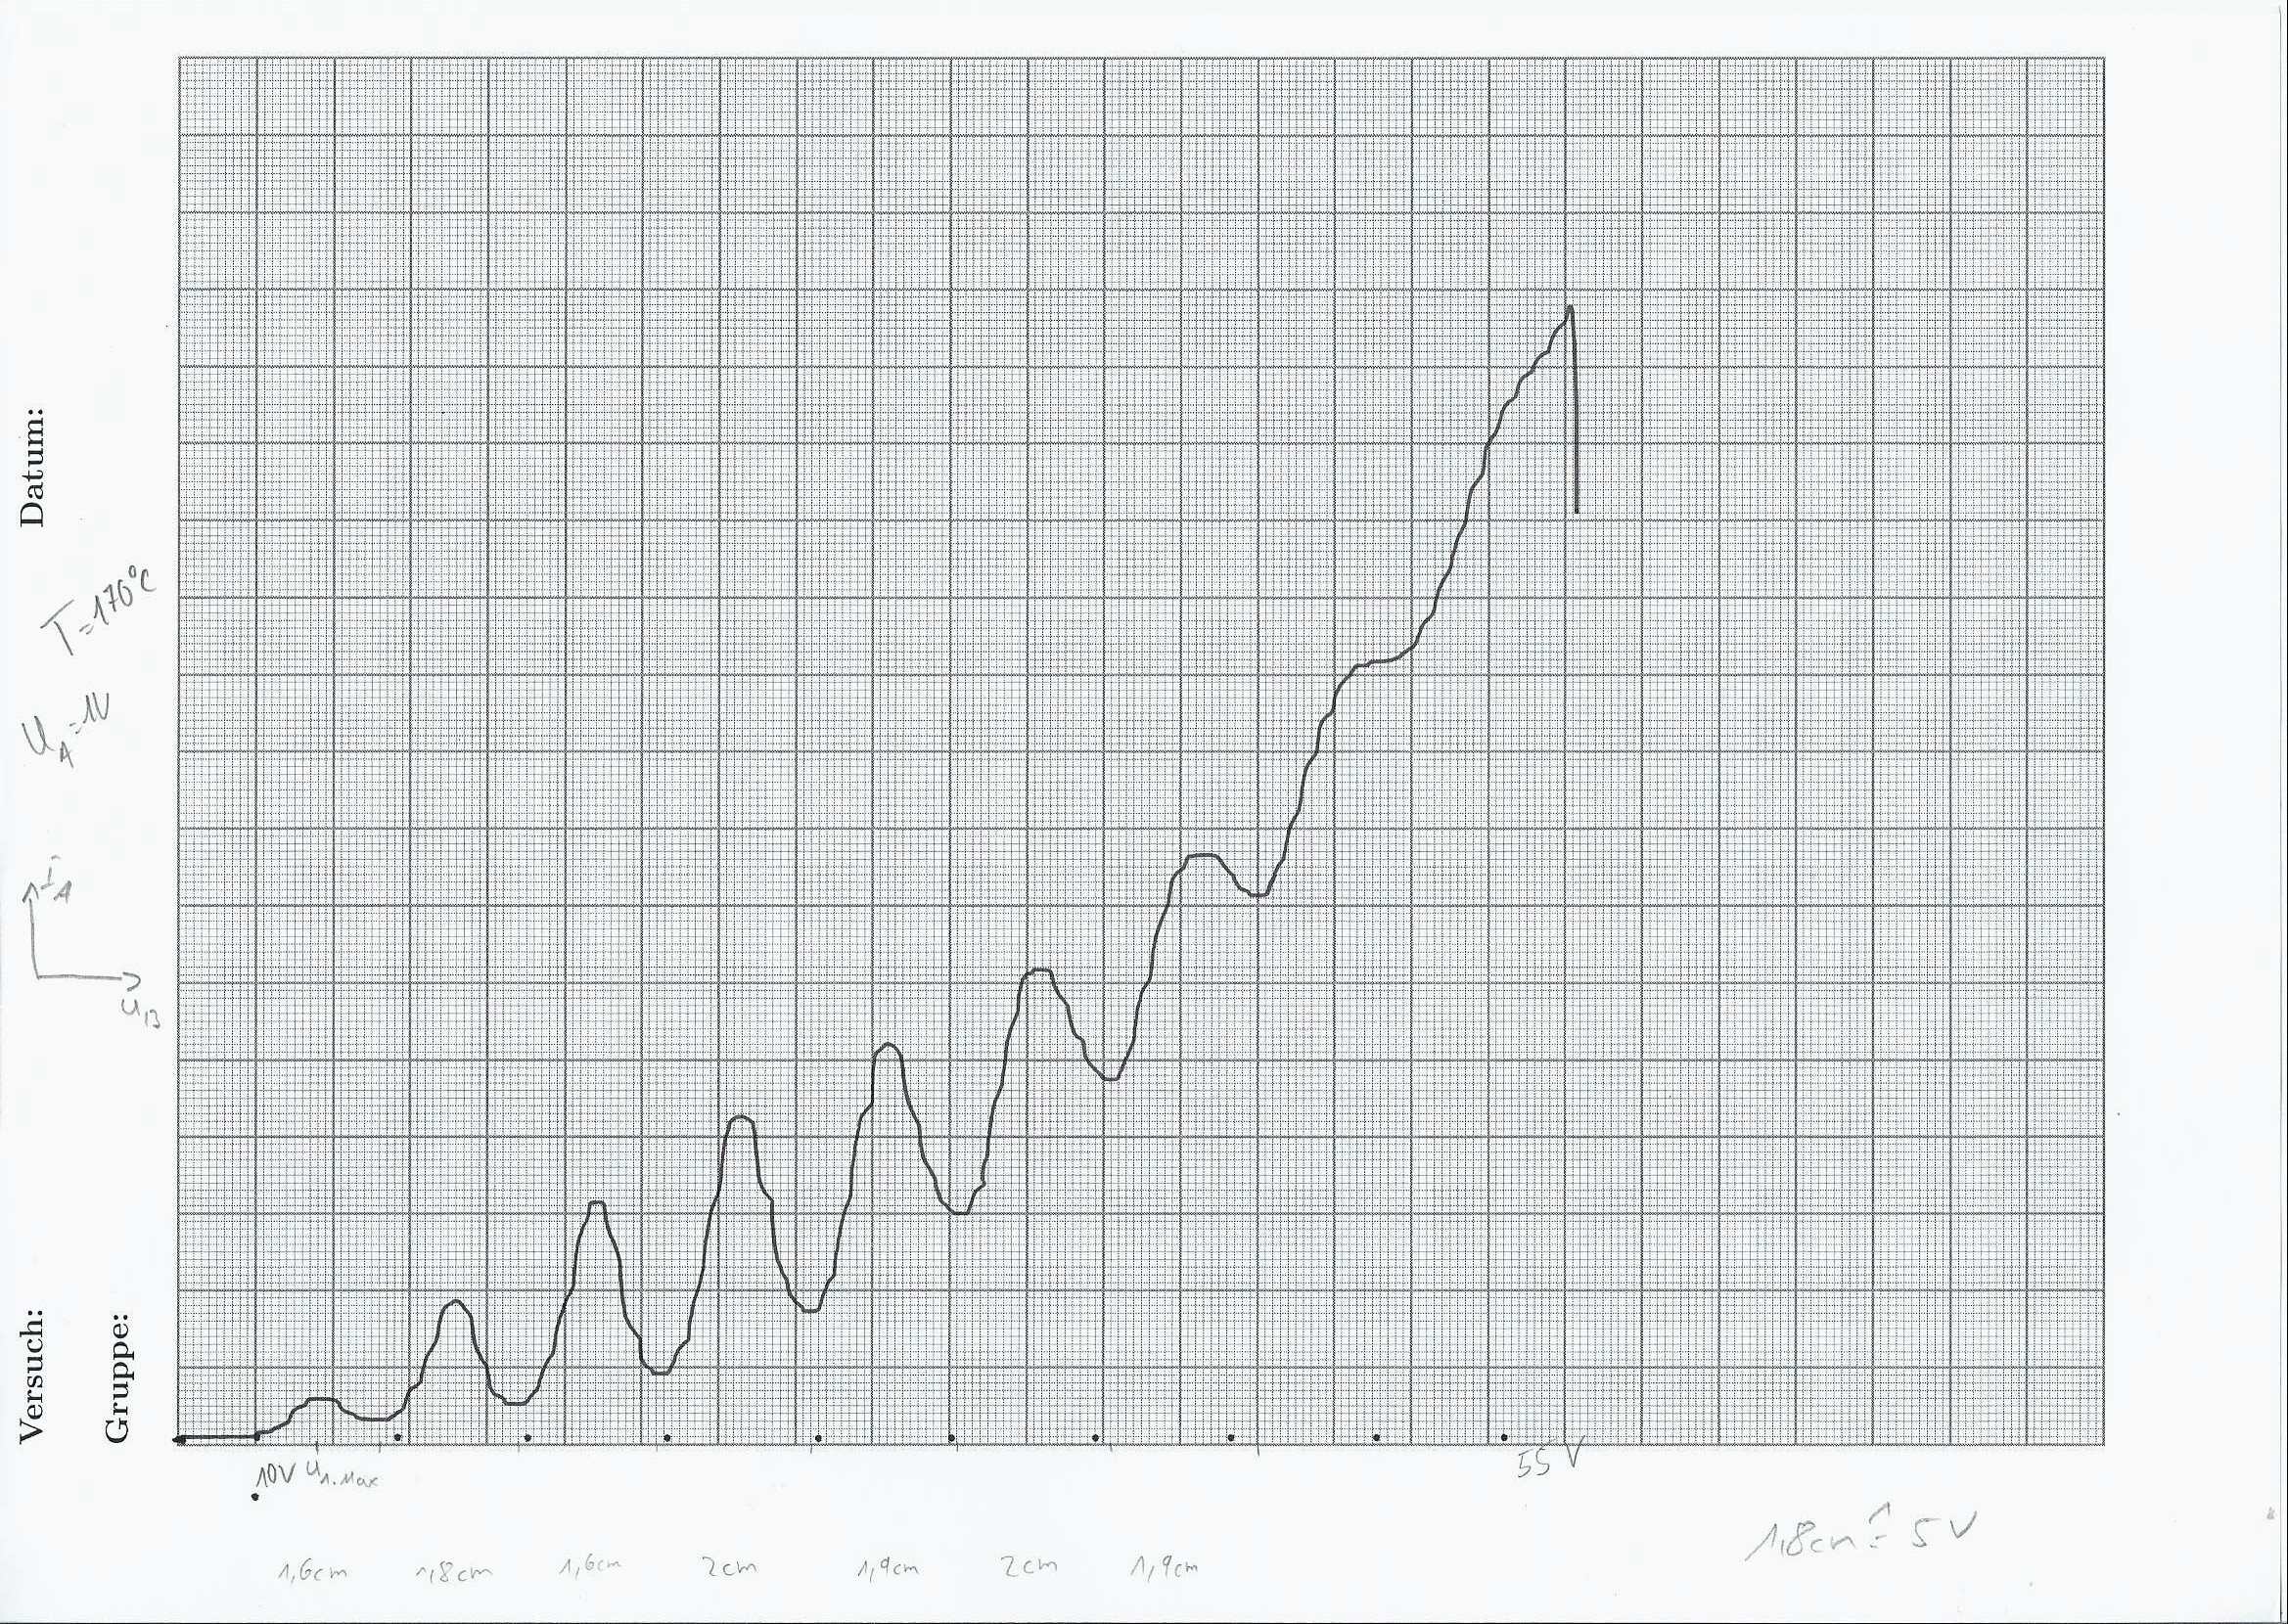
\includegraphics[width=0.8\textwidth]{bilder/kurve.pdf}
%   \caption{Frank-Hertz-Kurve zu Hg-Dampf}
%   \label{fig:kurve}
% \end{figure}
Die Temperatur wird auf $T=170\,\si{\degree}$ geregelt. Um die Anregungsenergien
$\Delta E$
des ersten Zustands von Hg zu bestimmen werden die Abstände der Minima $\zeta$ in
$\cm$ gemessen. Der Abstand zwischen zwei schwarzen Punkten entspricht
$1.8\cm = 5\Volt$. Mittels Dreisatz lassen sich so die jeweiligen $\Delta U$
Werte bestimmen. Mit
\begin{equation}
  \Delta E = e\cdot \Delta U
\end{equation}
ergeben sich die entsprechenden Energien. Alle benötigten Werte sind in Tabelle
\ref{tab:werte} zu finden.
\begin{table}
  \centering
  \begin{tabular}{c c}
    \toprule
    $\zeta \,/\cm$   & $\Delta E \,/\eV$  \\
    \midrule
    1.6 & 4.44 \\
    1.8 & 5.00 \\
    1.6 & 4.44 \\
    2.0 & 5.56 \\
    1.9 & 5.28 \\
    \bottomrule
  \end{tabular}
  \caption{Abstände $\zeta$ und Anregungsenergien $\Delta E$ des ersten Anregungszustands}
  \label{tab:werte}
\end{table}
Für den Mittelwert folgt:
\begin{equation*}
  \Delta E = (4.9 \pm 0.4) \eV.
\end{equation*}
Daraus lässt sich die Wellenlänge
\begin{equation*}
  \lambda = (250 \pm 20)\nm
\end{equation*}
mit der Gauß'schen Fehlerfortpflanzung
\begin{equation*}
  \Delta \lambda = \sqrt{\bigg(\frac{hc}{E^2}\bigg)^2\cdot \sigma_\su{\Delta E}^2}
\end{equation*}
berechnen.
